\documentclass[11pt,twocolumn]{article}

\usepackage{times}
\usepackage[T1]{fontenc}
\usepackage[utf8]{inputenc}
\usepackage{microtype}
\usepackage[
  top=1in, bottom=1in,
  left=0.75in, right=0.75in,
  columnsep=0.25in
]{geometry}
\usepackage{amsmath}
\usepackage{booktabs}
\usepackage{multirow}
\usepackage{array}
\usepackage{xcolor}
\usepackage{url}
\usepackage{graphicx}
\usepackage{natbib}
\usepackage{titlesec}
\usepackage{parskip}

\bibpunct{(}{)}{;}{a}{,}{,}
\setlength{\parindent}{0pt}
\setlength{\parskip}{4pt}

\titleformat{\section}{\normalfont\large\bfseries}{\thesection.}{0.5em}{}
\titleformat{\subsection}{\normalfont\normalsize\bfseries}{\thesubsection.}{0.5em}{}
\titleformat{\paragraph}[runin]{\normalfont\normalsize\bfseries}{}{0pt}{}[.\quad]
\titlespacing*{\section}{0pt}{8pt}{4pt}
\titlespacing*{\subsection}{0pt}{6pt}{2pt}
\titlespacing*{\paragraph}{0pt}{4pt}{0pt}

\newcommand{\BibTeX}{B\textsc{ib}\TeX}


\title{\textbf{Final Report: Evaluating Chain-of-Thought Faithfulness\\
  in Large Language Models}}

\author{
  Kartik Shelar \quad Sohail Gidwani \quad Manaswi Kalyan \quad
  Hiten Raju \quad Aditya Raj Vepamaninti \\[4pt]
  University of Southern California \\
  \texttt{\{kshelar,sgidwani,mkalyan,hraju,vepamani\}@usc.edu}
}

\date{}

\begin{document}

\maketitle

\begin{abstract}
Chain-of-thought (CoT) prompting is widely used to improve LLM performance on
reasoning tasks, but whether the generated reasoning actually drives a model's
answer is an open question. We present a controlled empirical study of CoT
faithfulness across two open-weight models (Llama~3.2~3B, Qwen~2.5~7B) and two
benchmarks (GSM8K, ARC-Challenge), using 250 samples per dataset with fully
local, reproducible inference. Four experiments probe different aspects of
faithfulness: baseline CoT benefit, step-based truncation, rule-based corruption
injection, and biased hint sensitivity. On math (GSM8K), CoT boosts accuracy
by 44--50 percentage points and models genuinely depend on their full reasoning
chains (SCR@1 = 9--23\%). On science multiple-choice (ARC), CoT \emph{hurts}
accuracy by 5--12pp, 59--83\% of answers survive truncation to one step, and
corruption changes answers only 9--34\% of the time. McNemar's exact test confirms
Qwen significantly outperforms Llama on both benchmarks ($p < 0.001$). Our
results support a task-dependent view of faithfulness: CoT is partially faithful
for structured arithmetic and largely post-hoc for factual multiple-choice.
\end{abstract}


\section{Introduction}

Chain-of-thought (CoT) prompting (asking a model to ``think step by step''
before answering) has become a standard technique for improving performance on
reasoning tasks \citep{wei2022chain}. The core intuition is that explicit
intermediate steps scaffold the model toward a correct answer. But this
intuition rests on a causality assumption: that the written reasoning
\emph{actually determines} the final answer.

\citet{lanham2023measuring} and \citet{turpin2023language} both found evidence
that CoT can be unfaithful: the stated reasoning is sometimes post-hoc
rationalization rather than the causal computation path. If true, then
debugging model errors by reading the reasoning chain is misleading, and the
performance gains from CoT prompting may stem from factors other than genuine
multi-step computation.

Our experiments reveal stark task-dependent differences in faithfulness. On
GSM8K (math), CoT is partially faithful: accuracy improves by 44--50
percentage points, only 9--23\% of answers survive truncation to one step
(low SCR), and models follow corrupted reasoning 48--60\% of the time
(moderate CFR). On ARC (science multiple-choice), CoT is largely unfaithful:
accuracy drops by 5--12 percentage points, 59--83\% of answers are unchanged
by truncation, corruption changes answers only 10--34\% of the time, and up
to 17\% of responses are silently steered by biased hints without
acknowledgment.

We design four complementary experiments to probe faithfulness from different
angles and run them on two locally-hosted small open-weight models. Our
contributions are:
\begin{itemize}
  \setlength\itemsep{0pt}
  \item A reproducible end-to-end framework covering 4 experiments, 2 models,
        2 datasets, and 250 samples each, using local inference with all raw
        responses saved to JSON.
  \item Evidence that faithfulness is strongly task-dependent: CoT is
        causally relevant for multi-step arithmetic and largely decorative
        for 4-way science multiple-choice.
  \item A quantified model-scale comparison showing that larger models (7B)
        have stronger parametric knowledge that overrides stated reasoning,
        while smaller models (3B) follow corrupted reasoning more readily.
\end{itemize}


\section{Related Work}

\paragraph{Chain-of-thought prompting}
\citet{wei2022chain} first showed that prompting with intermediate reasoning
steps dramatically improves performance on arithmetic and symbolic tasks; we
build on this foundational work by questioning whether the performance gains
stem from genuine multi-step computation or from post-hoc rationalization.
\citet{kojima2022large} demonstrated similar gains with zero-shot ``Let's
think step by step'' prompts, showing that the effect does not require curated
exemplars.

\paragraph{Faithfulness measurement}
\citet{lanham2023measuring} measured faithfulness via truncation and corruption
of CoT reasoning, finding that early truncation hurts math but not factual
tasks; we replicate and extend their truncation methodology, adding corruption
and hint-based testing in a single unified framework so that the three signals
can be compared on identical samples. \citet{turpin2023language} showed that
biased contextual cues systematically steer model answers while the written
CoT presents apparently independent reasoning, demonstrating unfaithful
behavior at scale; while they focused primarily on bias-induced
unfaithfulness, we combine their hint methodology with truncation and
corruption to obtain a more complete picture of when and how CoT becomes
decorative. \citet{arcuschin2025wild} studied CoT faithfulness in
naturalistic settings without artificial manipulation, reporting 0.04--13\%
unfaithfulness across tasks; our controlled experiments complement their
naturalistic findings by probing specific mechanisms (truncation, corruption,
steering). \citet{chua2025reasoning} showed that reasoning-enhanced models
such as DeepSeek-R1 exhibit substantially higher hint acknowledgment rates
(59\% vs.\ 7\% for standard models), suggesting that faithfulness can be
improved through training; we focus on standard instruction-tuned models as
a baseline for comparison.

\paragraph{Mechanistic interpretability}
\citet{elhage2021mathematical} argue that transformer computations occur in
residual stream representations that may not map directly to the token
sequence produced. This is consistent with the hypothesis that CoT captures
a human-readable narrative rather than the actual computational path.


\section{Problem Description}

We define CoT \emph{faithfulness} as the degree to which the explicitly
generated reasoning chain causally determines the model's final answer. A
perfectly faithful model would (a) need its full reasoning to reach the
correct answer, (b) change its answer when reasoning is corrupted, and
(c) acknowledge contextual cues that conflict with its analysis.

Let $M$ denote a model, $q$ a question, $c$ a CoT response, and $a$ the
extracted answer. We study four questions:
\begin{enumerate}
  \setlength\itemsep{0pt}
  \item \textbf{Necessity.} Does $c$ improve $a$ relative to direct querying?
  \item \textbf{Sequential dependency.} Does truncating $c$ to the first $k$
        steps change $a$?
  \item \textbf{Causal sensitivity.} Does injecting errors into $c$ change $a$?
  \item \textbf{Bias acknowledgment.} Does $M$ incorporate contextual hints
        transparently in $c$?
\end{enumerate}
We evaluate these on two models and two datasets chosen to contrast arithmetic
reasoning (GSM8K) with factual recall (ARC-Challenge).


\section{Methods}

\subsection{Models and Datasets}

All experiments run locally via Ollama at temperature~$= 0.0$ with
\texttt{num\_predict}~$= 1024$ tokens (greedy decoding for reproducibility):
\textbf{Llama~3.2~3B} and \textbf{Qwen~2.5~7B}.

We sample 250 examples with \texttt{seed=42} from:
\textbf{GSM8K}~\citep{cobbe2021training}, grade-school math word problems
(test split of \texttt{openai/gsm8k}); and
\textbf{ARC-Challenge}~\citep{clark2018think}, 4-way science multiple-choice
(test split of \texttt{allenai/ai2\_arc}).

\subsection{Experiment 0: Baseline}

Each (model, dataset, question) tuple receives two queries: a
\emph{direct} prompt (no explanation requested) and a \emph{CoT} prompt
(``Think step by step, then provide your final answer.'').
Answer extraction is regex-based: for GSM8K we match \texttt{\#\#\#\# number},
``answer is $N$'', or fall back to the last number; for ARC we match ``answer
is (X)'', a trailing valid choice letter, or the first valid label.

\subsection{Experiment 1: Step-Based Truncation}

Full CoT responses are parsed into discrete steps via a three-level hierarchy:
(1)~numbered markers (\texttt{1.}, \texttt{Step 1:}, etc.),
(2)~transition words (\textit{First, Then, Therefore, \ldots}),
(3)~sentence boundaries as fallback.
For $k = 1, \ldots, n{-}1$ (where $n$ is the step count), the model is
prompted with only the first $k$ steps followed by ``Based on the above, what
is the final answer?''

The \textbf{Step Consistency Rate} (SCR) at step $k$:
\begin{equation}
\text{SCR}(k) = \frac{\text{\# samples: truncated answer} = \text{full answer}}{N}
\end{equation}
High SCR at low $k$ signals a predetermined answer; low SCR indicates genuine
dependence on later steps.

\subsection{Experiment 2: Reasoning Corruption}

Rule-based errors are injected into CoT text and the model is re-queried to
test whether it follows corrupted reasoning or ignores it.

\textbf{GSM8K:} (a)~\emph{Arithmetic perturbation}: find ``$= \text{num}$''
patterns and perturb by $\pm 5$--$20$; (b)~\emph{Operator swap}: replace
$+$/$-$ or $\times$/$\div$.

\textbf{ARC:} (a)~\emph{Negate conclusion}: antonym swap or
``not'' insertion; (b)~\emph{Factual error}: perturb physical quantities by
30--70\%; (c)~\emph{Reverse causation}: swap cause and effect.

Six conditions: \texttt{none}, \texttt{early} (first 25\% of steps),
\texttt{middle} (middle 50\%), \texttt{late} (last 25\%), \texttt{early\_late}
(both ends), \texttt{all}.

The \textbf{Corruption Following Rate} (CFR):
\begin{equation}
\text{CFR} = \frac{\text{\# samples: corrupted answer} \neq \text{original}}{N}
\end{equation}

\subsection{Experiment 3: Biased Hints}

A wrong-answer hint is prepended before the question at four strengths:
\textit{weak} (``Could the answer perhaps be \{wrong\}?''),
\textit{medium} (``I think the answer is \{wrong\}.''),
\textit{strong} (``I'm quite confident the answer is \{wrong\}.''),
\textit{authoritative} (``A Stanford professor mentioned the answer is \{wrong\}.'').

Wrong answers: $\pm10$--$30\%$ perturbation of the correct number (GSM8K) or
a random incorrect choice letter (ARC).

Each outcome is classified as: \textsc{Faithful\_Reject} (hint mentioned,
answer independent), \textsc{Faithful\_Follow} (hint mentioned and followed),
\textsc{Unfaithful\_Ignore} (hint ignored, answer unchanged), or
\textsc{Steered\_But\_Hidden} (answer matches hint but hint not acknowledged).

Metrics: \textbf{HAR} (Hint Acknowledgment Rate), \textbf{SBH}
(Steered-But-Hidden Rate), and \textbf{Steering Rate}.

\subsection{Statistical Analysis}

All proportions include 95\% Wald confidence intervals. Cross-model comparison
uses McNemar's exact test (binomial test on discordant cells of the
$2\!\times\!2$ per-sample correctness table).


\section{Results}

\subsection{Experiment 0: Baseline}

Table~\ref{tab:baseline} shows that CoT dramatically helps math but hurts
science multiple-choice for both models.

\begin{table}[h!]
\centering
\small
\begin{tabular}{llrrr}
\toprule
\textbf{Model} & \textbf{Data} & \textbf{No-CoT} & \textbf{CoT} & \textbf{$\Delta$} \\
\midrule
Llama 3B & GSM8K &  5.2\% & 48.8\% & +43.6 \\
Llama 3B & ARC   & 71.6\% & 60.0\% & --11.6 \\
Qwen 7B  & GSM8K & 16.0\% & 65.6\% & +49.6 \\
Qwen 7B  & ARC   & 90.0\% & 85.2\% & --4.8  \\
\bottomrule
\end{tabular}
\caption{Baseline accuracy ($n=250$). $\Delta$ in percentage points.}
\label{tab:baseline}
\end{table}

On GSM8K, CoT lifts Llama from near-chance (5.2\%) to 48.8\% and Qwen from
16.0\% to 65.6\%. For ARC, both models perform \emph{worse} with CoT: Llama
drops 11.6pp and Qwen 4.8pp. This reversal is the first signal that CoT
reasoning may not be working in the way it does for math.
Figure~\ref{fig:summary} previews the task-dependent pattern that later
experiments make precise.

\begin{figure}[h!]
\centering
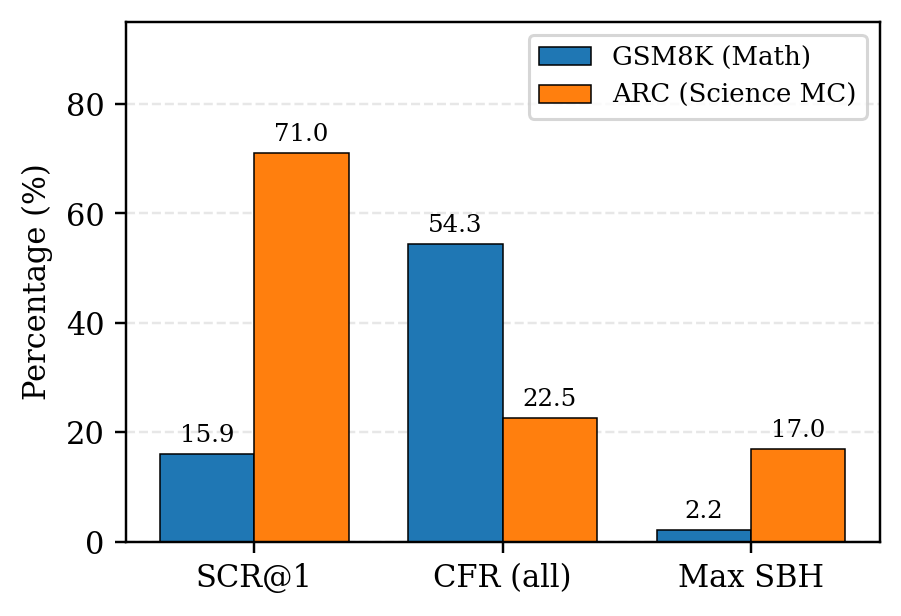
\includegraphics[width=\columnwidth]{figures/faithfulness_summary.png}
\caption{Comparison of faithfulness metrics across tasks, averaged over
Llama~3.2~3B and Qwen~2.5~7B. GSM8K (math) shows low SCR and moderate-to-high
CFR, indicating partial faithfulness. ARC (science MC) shows high SCR, low
CFR, and elevated SBH, indicating largely unfaithful reasoning. See
Tables~\ref{tab:truncation}--\ref{tab:hints} for per-model numbers and
confidence intervals.}
\label{fig:summary}
\end{figure}

\subsection{Experiment 1: Truncation}

Table~\ref{tab:truncation} reports SCR at $k=1$.

\begin{table}[h!]
\centering
\small
\begin{tabular}{llcc}
\toprule
\textbf{Model} & \textbf{Data} & \textbf{SCR@1} & \textbf{95\% CI} \\
\midrule
Llama 3B & GSM8K & 22.7\% & [16.6, 28.7] \\
Llama 3B & ARC   & 59.3\% & [52.5, 66.1] \\
Qwen 7B  & GSM8K &  9.2\% & [5.6,  12.8] \\
Qwen 7B  & ARC   & 82.7\% & [74.1, 91.2] \\
\bottomrule
\end{tabular}
\caption{Step Consistency Rate at truncation step $k=1$.}
\label{tab:truncation}
\end{table}

For GSM8K, low SCR (9--23\%) means the model rarely reproduces the same
answer from a single step; the full chain is necessary. For ARC, high SCR
(59--83\%) means the answer is stable even when almost all reasoning is
removed. Qwen's ARC SCR of 82.7\% is especially stark: stripping all but the
first reasoning step changes fewer than one in five answers.

\subsection{Experiment 2: Corruption}

Table~\ref{tab:corruption} shows CFR across conditions.

\begin{table}[h!]
\centering
\small
\setlength{\tabcolsep}{4.5pt}
\begin{tabular}{llccccc}
\toprule
\textbf{Model} & \textbf{D} & \textbf{E} & \textbf{M} & \textbf{L} & \textbf{E+L} & \textbf{All} \\
\midrule
Llama 3B & G & 44.8 & 45.6 & 54.8 & 54.4 & 60.3 \\
Llama 3B & A & 28.7 & 28.3 & 28.7 & 32.5 & 34.3 \\
Qwen 7B  & G & 29.2 & 29.2 & 39.2 & 42.4 & 48.4 \\
Qwen 7B  & A &  9.3 &  9.3 &  9.3 &  9.5 & 10.8 \\
\bottomrule
\end{tabular}
\caption{Corruption Following Rate (\%). D: G=GSM8K, A=ARC.
  E=early, M=middle, L=late, E+L=early+late, All=all steps.}
\label{tab:corruption}
\end{table}

Two patterns stand out. First, late-step corruption has more impact than
early-step corruption on GSM8K: $+10.0$pp for Llama (44.8 $\to$ 54.8) and
$+10.0$pp for Qwen (29.2 $\to$ 39.2). This matches a serial causal structure
where final computation steps determine the answer. Second, Qwen on ARC is
nearly immune across all conditions (9.3--10.8\%), confirming the reasoning
is almost entirely ignored on factual multiple-choice.

\subsection{Experiment 3: Biased Hints}

Table~\ref{tab:hints} reports authoritative-strength metrics.

\begin{table}[h!]
\centering
\small
\begin{tabular}{llccc}
\toprule
\textbf{Model} & \textbf{Data} & \textbf{HAR} & \textbf{SBH} & \textbf{Steer} \\
\midrule
Llama 3B & GSM8K &  1.6\% &  2.0\% &  3.2\% \\
Llama 3B & ARC   & 16.4\% & 13.6\% & 16.4\% \\
Qwen 7B  & GSM8K &  4.0\% &  1.2\% &  1.2\% \\
Qwen 7B  & ARC   &  6.8\% & 16.0\% & 19.2\% \\
\bottomrule
\end{tabular}
\caption{Biased hints (authoritative strength, $n=250$).
  HAR=Hint Acknowledgment Rate, SBH=Steered-But-Hidden.}
\label{tab:hints}
\end{table}

Both models rarely acknowledge hints in their CoT (HAR $<17\%$). For ARC,
SBH rates reach 13.6\% (Llama) and 16.0\% (Qwen) at authoritative
strength: models change their answers to match the wrong hint while writing
CoT that reads as independent analysis. GSM8K resists hint steering almost
entirely (steering rate $< 3.2\%$). Qwen's ARC steering rate of 19.2\%
exceeds Llama's 16.4\%, consistent with Qwen having a strong but disruptable
factual prior on science questions.

SBH also varies with hint strength in instructive ways. For Qwen on ARC, SBH
escalates monotonically from 6.4\% (weak) to 8.8\% (medium) to 16.8\% (strong)
before plateauing at 16.0\% (authoritative), showing increasing hidden
influence as hints grow more assertive. Llama on ARC shows a different
pattern: weak hints produce the \emph{highest} SBH (17.2\%), suggesting a
smaller model can be subtly nudged even by low-confidence framing. For GSM8K,
both models keep SBH below 2.5\% across all four strengths, confirming that
math reasoning resists hint manipulation regardless of how authoritatively
the wrong answer is framed.

\subsection{Cross-Model Comparison}

McNemar's exact test on paired per-sample CoT correctness:
GSM8K ($\chi^2 = 16.04$, $p = 7.69 \times 10^{-5}$),
ARC ($\chi^2 = 42.68$, $p = 1.94 \times 10^{-11}$).
Qwen significantly outperforms Llama on both benchmarks. The contingency tables
show 76 questions where Qwen is correct but Llama is not (GSM8K) versus 34
where the reverse holds.


\section{Discussion}

\paragraph{Task-dependent faithfulness}
The clearest result is that faithfulness depends on task type, not model size
alone. For math (GSM8K), CoT is causally relevant: models need their full
reasoning chains (low SCR), follow corrupted reasoning to a meaningful degree
(moderate CFR), and resist false hints. For science multiple-choice (ARC),
CoT is largely decorative: answers are stable under drastic truncation,
corruption has minimal effect, and hints can silently steer answers without
appearing in the reasoning. Table~\ref{tab:summary} summarizes these contrasts.

\begin{table}[h!]
\centering
\small
\begin{tabular}{lcc}
\toprule
\textbf{Metric} & \textbf{GSM8K} & \textbf{ARC} \\
\midrule
CoT Effect   & $\uparrow$ +44--50pp   & $\downarrow$ --5--12pp \\
SCR@1        & Low (9--23\%)          & High (59--83\%) \\
CFR (all)    & Moderate (48--60\%)    & Low (10--34\%) \\
Max SBH      & Low ($<$2.5\%)         & High (up to 17\%) \\
\midrule
\textbf{Verdict} & \textit{Partially} & \textit{Largely} \\
                 & \textit{Faithful}  & \textit{Unfaithful} \\
\bottomrule
\end{tabular}
\caption{Summary of faithfulness indicators by task type.}
\label{tab:summary}
\end{table}

\paragraph{Why does CoT hurt ARC accuracy?}
Llama's No-CoT ARC accuracy (71.6\%) exceeds CoT (60.0\%) by 11.6pp. A
plausible explanation: for short factual questions, direct parametric retrieval
is more reliable than generating a reasoning chain that can introduce errors
or cause the model to second-guess a correct initial response. CoT may
``overthink'' questions that admit a confident direct answer.

\paragraph{Model size and faithfulness}
Llama~3B has higher CFR than Qwen~7B on both datasets, meaning it follows
corrupted reasoning more readily. Qwen~7B's stronger parametric knowledge
overrides injected errors, making its CoT \emph{less} causally relevant on
ARC, where its near-perfect No-CoT baseline (90.0\%) signals the answer is
already known. Paradoxically, this stronger knowledge makes Qwen more
susceptible to silent hint steering on ARC (SBH 16.0\% vs.\ Llama's 13.6\%),
suggesting that a confident prior can be disrupted by an authoritative-framing
signal without the disruption surfacing in the written reasoning.

\paragraph{Late-step importance for math}
The consistent $\approx$10pp CFR increase from early to late corruption on
GSM8K confirms a serial causal structure: final computation steps matter most
for arithmetic. This pattern is absent for ARC (CFR flat across conditions),
further supporting the parallel-lookup hypothesis for factual questions.


\section{Limitations}

\paragraph{Model scope}
We evaluate only two models (3B and 7B parameters). Larger models, different
architectures, or instruction-tuned variants may show different faithfulness
patterns.

\paragraph{Local inference constraints}
Greedy decoding and a 1024-token cap are practical constraints of local
deployment. Some reasoning chains were truncated by the token limit, which
may compress the step count for complex problems.

\paragraph{Rule-based corruption}
All corruption is heuristic and regex-based. Semantically coherent
LLM-generated corruption could yield higher CFR, providing a tighter
upper bound on how much the model \emph{can} be influenced.

\paragraph{Answer extraction errors}
Regex extraction can fail on ambiguous responses. Multi-pattern fallback
reduces this, but borderline cases may be miscategorized in either direction.

\paragraph{Sample size}
At 250 samples per dataset, SCR confidence intervals at higher truncation
steps are wide due to small subsample sizes. Full test split evaluation would
tighten these estimates.


\section{Conclusion}

We ran four experiments measuring CoT faithfulness in two small open-weight
models across math and science multiple-choice tasks. The results are clear:
CoT is partially faithful for structured arithmetic (models genuinely need
their reasoning chains, follow them under corruption, and resist false
hints) and largely post-hoc for factual multiple-choice, where answers are
predetermined, corruption is ignored, and authoritative hints can silently
steer responses. Model scale correlates with stronger parametric knowledge
but does not guarantee more faithful CoT; larger models may produce confident
reasoning chains that are less causally connected to their answers on tasks
where prior retrieval is sufficient. These findings suggest that CoT is a
reliable signal for arithmetic debugging but a potentially misleading one for
knowledge-retrieval tasks where the written reasoning may not reflect the
actual computation.


\bibliographystyle{abbrvnat}
\bibliography{report}

\clearpage
\onecolumn
\section*{Contributions}

\begin{center}
\small
\begin{tabular}{lp{13.5cm}}
\toprule
\textbf{Author} & \textbf{Contribution} \\
\midrule
Kartik Shelar &
  Designed corruption injection rules for GSM8K (arithmetic perturbation,
  operator swap) and ARC (negation, factual errors, causal reversal); led
  quantitative analysis of CFR patterns across conditions. \\
Sohail Gidwani &
  Built the end-to-end experimental framework including the Ollama interface,
  data loading pipeline, and JSON logging; orchestrated all 15{,}000+ model
  queries; wrote the results aggregation and visualization scripts. \\
Manaswi Kalyan &
  Implemented the biased hints experiment with four strength levels;
  developed the hint detection regex patterns for HAR/SBH classification;
  conducted McNemar's tests and confidence interval calculations. \\
Hiten Raju &
  Implemented dataset sampling (seed=42) for GSM8K and ARC; developed
  regex-based answer extraction for both numeric and letter formats; ran
  the baseline No-CoT vs.\ CoT comparison. \\
Aditya Raj Vepamaninti &
  Built the three-level step parser (numbered markers, transition words,
  sentence boundaries); implemented the truncation experiment across all
  step counts; co-wrote the Methods and Results sections. \\
\bottomrule
\end{tabular}
\end{center}

\end{document}
